\documentclass{article}
\usepackage[utf8]{inputenc}
\usepackage{algorithm}
\usepackage{bbm}
\usepackage{amsmath}
\usepackage{amsthm}
\usepackage{amssymb}
\usepackage{multicol}
\usepackage{tabularx}
\usepackage[toc,page]{appendix}
\usepackage{verbatim}
\usepackage{tikz}
\usepackage{tkz-kiviat}

\usepackage{geometry}
 \geometry{
 a4paper,
 total={170mm,257mm},
 left=20mm,
 top=20mm,
 }

\title{Robust Signomial Programs}
\author{Ali Saab, Berk Ozturk}
\date{May 2017}

\setlength\parindent{0pt} % Removes all indentation from paragraphs

\renewcommand{\vec}{\mathbf}
\newcommand{\mat}{\mathbf}

\newtheorem{theorem}{Theorem}[section]
\newtheorem{corollary}{Corollary}[theorem]
\newtheorem{lemma}[theorem]{Lemma}
\newtheorem{proposition}[theorem]{Proposition}

\begin{document}

\maketitle

\begin{abstract}
TODO: Complete rework to frame around AC design. 

Signomial programming is useful in multidisciplinary non-convex optimization problems such as aircraft design. The formulation and solution of robust signomial programs (RSPs) would be beneficial since many parameters involved in these problems are prone to uncertainty, and can have significant effects on solution performance and feasibility. This paper proposes an approximate solution for an RSP leveraging an existing approximate robust geometric programming (RGP) formulation developed by Saab. The method is based on solving a sequence of RGPs, where each GP is a local approximation of the SP. Moreover, this paper also discusses the trade-off between robustness and optimality by implementing RSPs on a simple aircraft problem, and demonstrates how robust optimization affects aircraft design decisions.
\end{abstract}


\section*{Acronyms}
\begin{multicols}{2}
\begin{tabbing}
  XXXXXXX \= \kill% this line sets tab stop
$AR$ \> aspect ratio \\
$C_D$ \> drag coefficient \\ 
$C_{D_{A}}$ \> fuselage drag area \\ 
$C_L$ \> lift coefficient \\
$C_{L_{max}}$ \> lift coefficient at stall \\
GP \> geometric program \\
MDO \> multidisciplinary \\
    \>design optimization \\
$N_{ult}$ \> ultimate load factor \\
$Re$ \> Reynolds number \\
$S$ \> wing area \\ 
SP \> signomial program \\
$T_{flight}$ \> flight time \\
$W$ \> takeoff weight \\
$W_w$ \> wing weight \\
$W_{w_{strc}}$ \> wing structural weight \\
$W_{w_{surf}}$ \> wing skin weight\\
$V$ \> flight speed \\ 
$V_{f}$ \> fuel volume\\
$V_{f_{fuse}}$ \> fuel volume in the fuselage \\
$V_{f_{wing}}$ \> fuel volume in the wing \\
\end{tabbing}
\end{multicols}

\section{Introduction}

Robust optimization methods provide tractable methods to capture uncertainty in design.

TODO: Motivate the use of robust opt. for aircraft design over traditional methods, and stochastic/UQ. 

Geometric programs [GPs] are a method of log-convex optimization for which robust formulations exist. However, their stringent mathematical requirements limit their application in  non-log-convex problems. In this paper, we propose a tractable robust signomial program [RSP] which we solve as a sequential robust geometric program, allowing us to implement robustness in non-log-convex problems.

We implement the RSP formulation on a simple aircraft design problem with 19 free variables, 12 uncertain parameters and 17 constraints to demonstrate its potential. We believe that aircraft design problems can especially benefit from robustness. Oftentimes, aerospace engineers will implement margins in the design process to account for uncertainties in parameters that a design may be sensitive to, without explicit knowledge of the trade-off between robustness and optimality. A robust aircraft design formulation will allow designers to allocate margin more effectively to obtain better-performing designs with feasibility guarantees. 

\subsection{Geometric Programs}

Geometric programs are a method for log-convex optimization. They offer globally optimal solutions with no initial guesses, and allow engineers and designers to solve large-scale ($>$10,000 variables) nonlinear problems on the order of $\sim1$ second, given some stringent mathematical requirements. Given the general optimization problem below: 

\begin{align} 
\label{e:gpform}
\textrm{minimize } f_0(\mathbf{x}) & \nonumber \\
\textrm{subject to  } f_i(\mathbf{x}) &\leq 1, i=1,...,m \\
g_i (\mathbf{x}) &= 1, i = 1,...,p \nonumber
\end{align}

In a GP, $f_{i}$’s and $g_{i}$’s must have special posynomial and monomial forms below, with strictly positive coefficients:

A monomial is a function of the form 
\begin{equation}\label{e:monomial}
g(\mathbf{x}) = e^{\mathbf{a}\mathbf{x} + b}
\end{equation}
where $\mathbf{a} \in \mathbb{R}^n, b \in \mathbb{R}$ and $\mathbf{x} \in \mathbb{R}^n$. 

A posynomial is a function of the form
\begin{equation}\label{e:posynomial}
f(\mathbf{x}) = \sum_{k=1}^{K}e^{\mathbf{a}_k\mathbf{x} + b_k}
\end{equation}
where $\vec{a}_k \in \mathbb{R}^n, b_k \in \mathbb{R}$ and $\vec{x} \in \mathbb{R}^n$. A posynomial is a sum of monomials. Therefore, all monomials are also one-term posynomials.

Any monomial constraint $g(\vec{x}) = 1$ can be represented as $g(\vec{x}) \leq 1$ and $\frac{1}{g(\vec{x})} \leq 1$, therefore, the standard GP can be written in the inequality constrained form as follows:

\begin{equation}
\begin{aligned}
	& \text{minimize} && \textstyle{\sum}_{k=1}^{K_0}e^{\vec{a}_{0k}\vec{x} + b_{0k}} \\
	& \text{subject to} && \textstyle{\sum}_{k=1}^{K_i}e^{\vec{a}_{ik}\vec{x} + b_{ik}} \leq 1 \quad \forall i \in 1,...,m\\
\end{aligned}
\label{GP_inequality}
\end{equation}

A tractable approximation of robust GPs (RGPs) exists and will be discussed, and have been formulated with polyhedral and ellipsoidal uncertainty sets. RGPs allow for uncertainty in both the coefficients $b_k$ and the exponents $\mathbf{a}_{k}$. However, the restriction on the sign of the coefficients limits GPs (and consequently RGPs) to certain classes of problems. Signomials are constraints of the same form as $f(x)$, but allow for negative coefficients in $f(x)$. To be able to find robust solutions to signomial programs [SPs], we would like to create a framework to generalize the uncertainty sets used in RGPs to RSPs.

\subsection{Signomial Programs}

Signomials allow us to solve non-log-convex problems as sequential geometric programs. Signomials are a difference of posynomials shown in Equation~\ref{e:posynomial}. The log transform of an SP is not a convex optimization problem, but instead a difference of convex optimization problem that can be written in log-space as

\begin{equation}
\begin{aligned}
\text{minimize }f_{0}(\mathbf{x})& \\
\text{subject to }f_{i}(\mathbf{x}) -  h_{i}(\mathbf{x})& \leq 0, i = 1, ...., m \\
\end{aligned}
\end{equation}

where $f_{i}$ and $h_{i}$ are posynomials. This problem can be reliably solved iteratively by taking the monomial approximation of $g_{i}$ with a solution or initial guess $x_{i}$, solving this GP approximation to obtain a new solution $x_{i+1}$, and repeating the process until some convergence parameter is satisfied in the objective function.

The SP algorithm is well-studied, reliably solving SPs with an initial guess of all 1’s. SPs are guaranteed to be sub-optimal but feasible solutions to a general non-linear problem. 


\section{Approach to Solving RSPs}

Our approach to solving the RSP is the following: 

\begin{enumerate}
    \item Solve the SP with no uncertainty, initialized by a vector of 1's. We call this solution $x_0$.
    \item Solve the SP with a chosen uncertainty set, using $x_0$ as the initial guess. 
\end{enumerate}

Step 2 requires the retuning of the SP algorithm as follows:
\newline
\newline
Initialize $x_0 = \vec{1}$ \newline
 While $reltol \geq 1e-4$:
    \begin{enumerate}
        \item Substitute $x_i$ as the initial guess to the SP. 
        \item Find the RGP approximation to the SP with guess $x_i$.
        \item Solve the RGP to obtain $x_{i+1}$. 
        \item Calculate $reltol$.
    \end{enumerate}

$reltol$ is the relative change in the objective function value for the GP. The RSP algorithm solves reliably for a range of $reltol$s, but a value of $1e-4$ was chosen for the models evaluated in this paper. 


\section{RGPs}
This part is commented because it repeats the Robust Geometric Programming stuff from the first paper
\begin{comment}
\subsection{Decoupled Form}
WOLG the objective function could be assumed linear (one dimensional variable) and deprived of any data (epigraph formulation), therefore the cost will be ignored throughout this report. Moreover, the GP will be represented as follows

\begin{equation}
\begin{aligned}
\textstyle{\sum}_{k=1}^{K_i}e^{\vec{a}_{ik}\vec{x} + b_{ik}} &\leq 1 &&\forall i \in \mathbf{P}\\
e^{\vec{a}_{i1}\vec{x} + b_{i1}} + e^{\vec{a}_{i2}\vec{x} + b_{i2}} &\leq 1 &&\forall i \in \mathbf{M}\\
e^{\vec{a}_{i1}\vec{x} + b_{i1}} &\leq 1 &&\forall i \in \mathbf{N}
\end{aligned}
\label{GP_decoupled}
\end{equation}

where 
\begin{itemize} 
	\item $\mathbf{P}$ = $\left\{i : \vec{K}_i > 2\right\}$
	\item $\mathbf{N}$ = $\left\{i : \vec{K}_i = 2\right\}$		
	\item $\mathbf{M}$ = $\left\{i : \vec{K}_i = 1\right\}$
\end{itemize}

%In words, the constraints are classified into three groups
%\begin{itemize}
%	\item Three or more term posynomials which are referred to by the set $\mathbf{P}$
%	\item Two term posynomials which are referred to by the set $\mathbf{N}$	
%	\item Monomials (one term posynomials) which are referred to by the set $\mathbf{M}$	
%\end{itemize}
%\nomenclature{$\vec{t}$}{vector of artificial variables ($\textstyle{\sum_{i \in N} \vec{K}_i} \times 1$)}
%\nomenclature{$t_{ik}$}{the variable replacing the $k^{th}$ monomial in the $i^{th}$ posynomail}
The GP in equation \eqref{GP_decoupled} in convex form is represented as follows

\begin{equation}
\begin{aligned}
\log(\textstyle{\sum}_{k=1}^{K_i}e^{\vec{a}_{ik}\vec{x} + b_{ik}}) &\leq 0 &&\forall i \in \mathbf{P} \\
\log(e^{\vec{a}_{i1}\vec{x} + b_{i1}} + e^{\vec{a}_{i2}\vec{x} + b_{i2}}) &\leq 0 &&\forall i \in \mathbf{N} \\
\vec{a}_{i1}\vec{x} + b_{i1} &\leq 0 &&\forall i \in \mathbf{M}
\end{aligned}
\label{GP_convex}
\end{equation}
\subsection{Robust Counterpart}
In robust optimization, a formulation that is immune to the uncertainty in the system's data should be derived. The data will be assumed living in an uncertainty set $\mathcal{U}$, where $\mathcal{U}$ is parameterized affinly by a perturbation vector $\vec{\zeta}$ as follows
\begin{equation}
	\mathcal{U} = \left\{[\mat{A};\vec{b}] = [\mat{A}^0;\vec{b}^0] + \textstyle{\sum_{l=1}^{L}\zeta_l[\mat{A}^l;\vec{b}^l]}\right\}
	\label{Data}
\end{equation}
where $\vec{\zeta}$ belongs to some perturbation set $\mathcal{Z} \in \mathbb{R}^L$ such that
\begin{equation}
	\mathcal{Z} = \left\{ \vec{\zeta} \in \mathbb{R}^L: \exists \vec{u} \in \mathbb{R}^k:\mat{P}\vec{\zeta} + \mat{Q}\vec{u} + \vec{p} \in \textbf{K} \right\}
	\label{perturbation_set}
\end{equation}

The robust counterpart of the uncertain geometric program given by equation \eqref{GP_decoupled} is

\begin{multicols}{2}
\begin{equation}
\begin{aligned}
\textstyle{\sum}_{k=1}^{K_i}e^{\vec{a}_{ik}\vec{x} + b_{ik}} &\leq 1 &&\forall i \in \mathbf{P} && \forall \vec{\zeta} \in \mathcal{Z}\\
e^{\vec{a}_{i1}\vec{x} + b_{i1}} + e^{\vec{a}_{i2}\vec{x} + b_{i2}} &\leq 1 &&\forall i \in \mathbf{M} && \forall \vec{\zeta} \in \mathcal{Z}\\
e^{\vec{a}_{i1}\vec{x} + b_{i1}} &\leq 1 &&\forall i \in \mathbf{N} && \forall \vec{\zeta} \in \mathcal{Z}.
\end{aligned}
\label{GP_counterparts}
\end{equation}\break
%$\iff$  
%\break
\begin{equation}
\begin{aligned}
&\max_{\vec{\zeta} \in \mathcal{Z}} \left\{\textstyle{\sum}_{k=1}^{K_i}e^{\vec{a}_{ik}\vec{x} + b_{ik}}\right\} &&\leq 1 &&\forall i \in \mathbf{P}\\
&\max_{\vec{\zeta} \in \mathcal{Z}} \left\{e^{\vec{a}_{i1}\vec{x} + b_{i1}} + e^{\vec{a}_{i2}\vec{x} + b_{i2}}\right\} &&\leq 1 &&\forall i \in \mathbf{M}\\
&\max_{\vec{\zeta} \in \mathcal{Z}} \left\{e^{\vec{a}_{i1}\vec{x} + b_{i1}}\right\} &&\leq 1 &&\forall i \in \mathbf{N}
\end{aligned}
\label{GP_counterparts_finite}
\end{equation}
\end{multicols}

The above two sets of constraints state that the robust optimal solution should be feasible for all possible realizations of the perturbation vector $\vec{\zeta}$. Unfortunately, the robust counterpart of a geometric program is intractable using current solvers. Throughout this report, an approximate formulation will be derived using robust linear programming.\\ [12pt]

\subsection{Conservative Tractable Formulation} \label{Conservative}
Since it is intractable to solve a robust geometric program, this section will discuss a simple approximate formulation of the robust counterparts given by \eqref{GP_counterparts_finite}.\\[12pt]
The constraints corresponding to the set $\mathbf{M}$ of constraints are linear and therefore tractable, as a result, we should deal with the sets $\mathbf{P}$ and $\mathbf{N}$ only.\\[12pt]
The fact that $\max_{\vec{\zeta} \in \mathcal{Z}} \left\{\textstyle{\sum}_{k=1}^{K_i}e^{\vec{a}_{ik}\vec{x} + b_{ik}}\right\} \leq \sum_{k=1}^{K_i}\max_{\vec{\zeta} \in \mathcal{Z}} \left\{e^{\vec{a}_{ik}\vec{x} + b_{ik}}\right\}$ suggests the following safe constraints for the constraints corresponding to elements in $\mathbf{P}$ and $\mathbf{N}$
\begin{equation}
	\sum_{k=1}^{K_i}\max_{\vec{\zeta} \in \mathcal{Z}} \left\{e^{\vec{a}_{ik}\vec{x} + b_{ik}}\right\} \leq 1
	\label{conservative_robust_constraint}
\end{equation}
Equation \eqref{conservative_robust_constraint} suggests the following "conservative" formulation of the robust counterpart for the uncertain geometric program
\begin{equation}
\begin{aligned}
&\textstyle{\sum}_{k=1}^{K_i}\max_{\vec{\zeta} \in \mathcal{Z}} \left\{e^{\vec{a}_{ik}\vec{x} + b_{ik}}\right\} &&\leq 1 &&\forall i \in \mathbf{P},\mathbf{M}\\
&\max_{\vec{\zeta} \in \mathcal{Z}} \left\{e^{\vec{a}_{i1}\vec{x} + b_{i1}}\right\} &&\leq 1 &&\forall i \in \mathbf{N}
\end{aligned}
\label{GP_safe_conservative}
\end{equation}

which is equivalent to

\begin{equation}
\begin{aligned}
&\textstyle{\sum}_{k=1}^{K_i}t_{ik} &&\leq 1 &&\forall i \in \mathbf{P},\mathbf{M} \\
&\max_{\vec{\zeta} \in \mathcal{Z}} \left\{e^{\vec{a}_{ik}\vec{x} + b_{ik}}\right\} &&\leq t_{ik} &&\forall i \in \mathbf{P},\mathbf{M} &&\forall k \in 1,...,K_i\\
&\max_{\vec{\zeta} \in \mathcal{Z}} \left\{e^{\vec{a}_{i1}\vec{x} + b_{i1}}\right\} &&\leq 1 &&\forall i \in \mathbf{N}
\end{aligned}
\label{GP_safe_decoupled}
\end{equation}

In log-space, Equation \eqref{GP_safe_decoupled} is

\begin{equation}
\begin{aligned}
&\log(\textstyle{\sum}_{k=1}^{K_i}e^{s_{ik}}) &&\leq 0 &&\forall i \in \mathbf{P},\mathbf{M} \\
&\max_{\vec{\zeta} \in \mathcal{Z}} \left\{\vec{a}_{ik}\vec{x} + b_{ik}\right\} &&\leq s_{ik} &&\forall i \in \mathbf{P},\mathbf{M} &&\forall k \in 1,...,\vec{K}_i\\
&\max_{\vec{\zeta} \in \mathcal{Z}} \left\{\vec{a}_{i1}\vec{x} + b_{i1}\right\} &&\leq 0 &&\forall i \in \mathbf{N}
\end{aligned}
\label{GP_safe_convex}
\end{equation}

It can be observed that the convex constraints in equation \eqref{GP_safe_convex} are deprived of data and uncertainty is only present in the linear constraints. As a result, this problem is tractable using robust linear programming.\\[12pt]
Although this formulation might seem too conservative for some problems due to the fact that monomials are being decoupled, however, it is exact for a wide range of problems that satisfy the following criteria
\begin{itemize}
	\item $C_1$: The perturbation set is independent, e.g. $\mathcal{Z} = \left\{ \vec{\zeta} \in \mathbb{R}^L: \|\vec{\zeta}\|_{\infty} \leq \Gamma\right\}$
	\item $C_2$: The monomials in each posynomial are independent, and if dependence only exists between the $'b'$s, then it should be "good" dependence, e.g. if $b_{11} = b_{11}^0 + \zeta_1$, $b_{12} = b_{12}^0 + \zeta_1 - \zeta_2$, and $b_{13} = b_{13}^0 + \zeta_2$, then $b_{11}$ and $b_{12}$ are dependent, but the dependence is good since the sign of the coefficients multiplied by the perturbation $\zeta_1$ are the same. However, $b_{12}$ and $b_{13}$ are dependent, but in a bad way due to the fact that the signs of the coefficients multiplied by the perturbation $\zeta_2$ are different
\end{itemize}
When $C_1$ and $C_2$ are satisfied for the $i^{th}$ posynomial, then
$$
\max_{\vec{\zeta} \in \mathcal{Z}} \left\{\textstyle{\sum}_{k=1}^{K_i}e^{\vec{a}_{ik}\vec{x} + b_{ik}}\right\} = \sum_{k=1}^{K_i}\max_{\vec{\zeta} \in \mathcal{Z}} \left\{e^{\vec{a}_{ik}\vec{x} + b_{ik}}\right\}
$$
and the "conservative" formulation is no longer conservative, but exact.\\

\subsection{Robust Two Term Posynomials} \label{twoTerm}
The focus now will be on modifying the methodology provided in section \ref{Conservative} so that the solution is less conservative. This section will review Boyd's work on approximating two term posynomials in log-space using piece-wise linear functions \footnote{ Kan-Lin Hsiung, Seung-Jean Kim, and Stephen Boyd. Tractable approximate robust geometric programming. \textit{Optimization and Engineering}, 9(2):95118, Apr 2007}.\\[12pt] 
Consider the convex function $\phi(x) = \log(1 + e^x)$, then the unique best r-term piece-wise linear convex lower approximation of $\phi$ is
\begin{equation}
\underline{\phi}_r = 
\begin{cases}
0 \qquad &\text{if} \qquad x \in (- \infty, x_1]\\
\underline{a}_ix + \underline{b}_i &\text{if} \qquad x \in [x_i, x_{i+1}], i=1,2,..,r-2\\
x &\text{if} \qquad x \in [x_{r-1}, \infty)
\end{cases}
\label{lower_phi}
\end{equation}
such that
\begin{itemize}
	\item $x_1 < x_2 < ... < x_{r-1}$
	\item $\underline{a}_0 = 0 < \underline{a}_1 < \underline{a}_2 < ... < \underline{a}_{r-2} < \underline{a}_{r-1} = 1$
	\item $\underline{a}_i + \underline{a}_{r-i-1} = 1\quad \forall i \in \left\{0,1, ..., r-1\right\}$
	\item $\underline{b}_i = \underline{b}_{r-i-1} \quad \forall i \in \left\{1, ..., r-2\right\}$
	\item $\underline{b}_0 = \underline{b}_{r-1} = 0$
\end{itemize}
Moreover, $\exists$ $\tilde{x}_1, \tilde{x}_2, ..., \tilde{x}_{r-2} \in \mathbf{R}$ satisfying
$$
x_1 < \tilde{x}_1 < x_2 < \tilde{x}_2 < ... < x_{r-2} < \tilde{x}_{r-2} < x_{r-1}
$$
such that $\underline{a}_ix + \underline{b}_i$ is tangent to $\phi$ at $\tilde{x}_i$.\\
Finally, the maximum approximation error $\epsilon_r$ of this piece-wise linearization occurs at the break points $x_1, ..., x_{r-1}$. The piece-wise linearization above will be used in approximating two term posynomials using piece-wise linear functions.\\[12pt]
Let $h= \log(e^{y_1} + e^{y_2})$ be a two term posynomial in log-space, where $y_1 = \vec{a}_1\vec{x} + b_1$ and $y_2 = \vec{a}_2\vec{x} + b_2$, then the unique best r-term piece-wise linear lower approximation is 
\begin{equation}
\begin{aligned}
\underline{h_r} = max\left\{&\underline{a}_{r-1}y_1 + \underline{a}_0y_2 + \underline{b}_0,\right. \underline{a}_{r-2}y_1 + \underline{a}_1y_2 + \underline{b}_1, \underline{a}_{r-3}y_1 + \underline{a}_2y_2 + \underline{b}_2,  \\
&\left. ..., \underline{a}_{1}y_1 + \underline{a}_{r-2}y_2 + \underline{b}_{r-2}, \underline{a}_0y_1 + \underline{a}_{r-1}y_2 + \underline{b}_{r-1}\right\}
\end{aligned}
\end{equation}
while its unique best r-term piece-wise linear upper approximation is 
\begin{equation}
\overline{h_r} = \underline{h_r} + \epsilon_r
\end{equation}
where $\underline{a}_{0}, \underline{a}_{1}, \underline{a}_{2}, ..., \underline{a}_{r-2}$ and $\underline{b}_{1}, \underline{b}_{2}, ..., \underline{b}_{r-2}, \underline{a}_{r-1}$ are as given in equation \eqref{lower_phi}, and $\epsilon_r$ is the maximum error between $\phi$ and $\underline{\phi}_r$.\\[12pt]
As a result, we know that $\overline{h}_r \geq h$, and therefore each posynomial in the set $\mathbf{N}$ is replaced by its best r-term piece-wise linear upper approximation (a safe approximation).\\[12pt]
This methodology needs to throw a sufficient number of constraints if a less conservative solution (better than the previous formulation) is to be achieved, however, it accounts for any dependency between the two monomials in a two term posynomial, and the problem will become tractable since a piece-wise linear constraint could be represented as a set of linear constraints.\\[12pt]

\subsection{Robust Large Term Posynomials}\label{k_term}
After taking care of the monomials and two term posynomials in a GP, its time to deal with the posynomial constraints corresponding to the set $\mathbf{P}$.\\[12pt] 
The first step is to divide the large posynomial into smaller posynomials if possible. To do so, consider the set $\mathbf{I}_i$ associated with a large posynomial $p_i$, $i \in \mathbf{P}$ where 
\begin{equation}
\mathbf{I}_i = \left\{ 1,2,...,K_i\right\} 
\label{monomials_set}
\end{equation}
Then define an equivalence relation $\mathcal{R}$ on the set $\mathbf{I}_i$ where
\begin{equation}
\mathcal{R} = \left\{k_1 \sim k_2 \iff e^{\vec{a}_{ik_1}\vec{x} + b_{ik_1}} \text{ and } e^{\vec{a}_{ik_2}\vec{x} + b_{ik_2}} \text{ are directly or indirectly dependent} \right\}
\label{equivalence_relation}
\end{equation}
It is clear that $\mathcal{R}$ is an equivalence relation, therefore, when applied on $\mathbf{I}_i$, $\mathbf{I}_i$ would split into equivalence classes $S_{i,1}, S_{i,2}, ..., S_{i,N_e^i}$, $N_e^i \leq K_i$, then
$$
\max_{\vec{\zeta} \in \mathcal{Z}} \left\{\textstyle{\sum}_{k=1}^{K_i}e^{\vec{a}_{ik}\vec{x} + b_{ik}}\right\} = \textstyle{\sum}_{j=1}^{N_e^i} \max_{\vec{\zeta} \in \mathcal{Z}} \left\{\textstyle{\sum}_{k \in S_{i,j}}e^{\vec{a}_{ik}\vec{x} + b_{ik}}\right\}
$$
and therefore, the constraints corresponding to $\mathbf{P}$ in equation \eqref{GP_counterparts_finite} will be replaced by the following equivalent set of constraints
\begin{equation}
\begin{aligned}
\textstyle{\sum}_{j=1}^{N_e^i} t_{ij} &\leq 1 \qquad &&\forall i \in \mathbf{P}\\
\max_{\vec{\zeta} \in \mathcal{Z}} \left\{\textstyle{\sum}_{k \in S_{i,j}} e^{\vec{a}_{ik}\vec{x} + b_{ik}} \right\} &\leq t_{ij} &&\forall i \in \mathbf{P} \qquad &&\forall j = 1, ..., N_e^i\\
\end{aligned}
\label{equivalent_class_setP}
\end{equation}

Let 
\begin{itemize}
	\item $\mathbf{P_i'} = \left\{j:|S_{i,j}| \geq 3\right\}$ $\rightarrow$ intractable
	\item $\mathbf{M_i'} = \left\{j:|S_{i,j}| = 2\right\}$ $\rightarrow$ tractable
	\item $\mathbf{N_i'} = \left\{j:|S_{i,j}| = 1\right\}$ $\rightarrow$ tractable
\end{itemize}
Let $S_{i,j}^k$ be the $k^{th}$ element of $S_{i,j}$, and let $\mathcal{L}_{i,j}^k$ be the monomial $\vec{a}_{iS_{i,j}^k}\vec{x} + b_{iS_{i,j}^k}$, then \eqref{equivalent_class_setP} is equivalent to
\begin{equation}
\begin{aligned}
&\textstyle{\sum}_{j=1}^{N_e^i} t_{ij} &&\leq 1 \qquad &&\forall i \in \mathbf{P}\\
&\max_{\vec{\zeta} \in \mathcal{Z}} \left\{\textstyle{\sum}_{k=1}^{|S_{i,j}|} e^{\mathcal{L}_{i,j}^k} \right\} &&\leq t_{ij} &&\forall i \in \mathbf{P} \qquad &&\forall j \in \mathbf{P_i'}\\
&\max_{\vec{\zeta} \in \mathcal{Z}} \left\{e^{\mathcal{L}_{i,j}^1} + e^{\mathcal{L}_{i,j}^2} \right\} &&\leq t_{ij} &&\forall i \in \mathbf{P} \qquad &&\forall j \in \mathbf{M_i'}\\
&\max_{\vec{\zeta} \in \mathcal{Z}} \left\{e^{\mathcal{L}_{i,j}^1} \right\} &&\leq t_{ij} &&\forall i \in \mathbf{P} \qquad &&\forall j \in \mathbf{N_i'}
\end{aligned}
\label{equivalent_class_setP_separated}
\end{equation}

When most of the monomials are certain, or when the the perturbation set is independent, the large posynomials would certainly be reduced into several smaller posynomials, and in some cases into monomials.\\[12pt]
The discussion regarding large posynomial approximation will be divided into two parts
\begin{enumerate}
	\item Robust large posynomials with uncertain coefficients $\vec{b}$ and certain exponents $\mat{A}$
	\item Robust large posynomials with uncertain coefficients and exponents.
\end{enumerate}

\subsection{Uncertain Coefficients Only}
The exponents in many applications regarding geometric programming are certain, therefore it is interesting to look at the problem where only the $'b'$s are uncertain and are given by
$$
\vec{b} = \vec{b}^0 + \textstyle{\sum}_{l=1}^{L}\vec{b}^l\zeta_l
$$
where $\vec{\zeta} \in \mathcal{Z}$ as given by equation \eqref{perturbation_set}.\\
Consider the second set of constraints of equation \eqref{equivalent_class_setP_separated}, and note that 
$$
\begin{aligned}
&\max_{\vec{\zeta} \in \mathcal{Z}} \left\{\textstyle{\sum}_{k=1}^{|S_{i,j}|} e^{\vec{a}_{iS_{i,j}^k}\vec{x} + b_{iS_{i,j}^k}} \right\} &&\leq t_{ij} &&\forall i \in \mathbf{P} \qquad &&\forall j \in \mathbf{P_i'}\\
\Leftrightarrow &\max_{\vec{\zeta} \in \mathcal{Z}} \left\{\textstyle{\sum}_{k=1}^{|S_{i,j}|} e^{\vec{a}_{iS_{i,j}^k}\vec{x} + b^0_{iS_{i,j}^k}}e^{\textstyle{\sum}_{l=1}^{L}b^l_{iS_{i,j}^k}\zeta_l} \right\} &&\leq t_{ij} &&\forall i \in \mathbf{P} \qquad &&\forall j \in \mathbf{P_i'}\\
\Leftrightarrow &\max_{\vec{\zeta} \in \mathcal{Z}} \left\{\textstyle{\sum}_{k=1}^{|S_{i,j}|}\textstyle{\prod}_{l=1}^{L}e^{b^l_{iS_{i,j}^k}\zeta_l} e^{\vec{a}_{iS_j^i(k)}\vec{x} + b^0_{iS_{i,j}^k}} \right\} &&\leq t_{ij} &&\forall i \in \mathbf{P} \qquad &&\forall j \in \mathbf{P_i'}\\
\end{aligned}
$$
The above constraint could be thought of as an uncertain linear constraint in terms of the variables $v_{i,j}^k = e^{\vec{a}_{iS_{i,j}^k}\vec{x} + b^0_{iS_{i,j}^k}}$ for $k = 1,...,|S_{i,j}|$ as follows
\begin{equation}
\max_{\vec{\zeta} \in \mathcal{Z}} \left\{\textstyle{\sum}_{k=1}^{|S_{i,j}|}\left(\textstyle{\prod}_{l=1}^{L}e^{b^l_{iS_{i,j}^k}\zeta_l}\right) v_{i,j}^k \right\} \leq t_{ij} \qquad \forall i \in \mathbf{P} \qquad \forall j \in \mathbf{P_i'}
\label{linearCon_expPerts}
\end{equation}
Although the constraints are linear in terms of $\vec{v_j^i}$, the perturbations are not affine but exponential. And since it is hard to deal with exponential perturbations, then it might be more convenient to linearize the perturbations.

\subsubsection{Linearizing perturbations}
Although the perturbations are not affine, however, they have some nice property which is convexity. This implies that there exists some half-space (affine function) $[\vec{f}_{i,j}^k]^T\vec{\zeta} + g_{i,j}^k \geq \textstyle{\prod}_{l=1}^{L}e^{b^l_{iS_{i,j}^k}\zeta_l}$. Therefore, a safe approximation of the constraints in equation \eqref{linearCon_expPerts} is
\begin{equation}
\max_{\vec{\zeta} \in \mathcal{Z}} \left\{\textstyle{\sum}_{k=1}^{|S_{i,j}|}\left([\vec{f}_{i,j}^k]^T\vec{\zeta}\right)v_{i,j}^k \right\} + \textstyle{\sum}_{k=1}^{|S_{i,j}|}g_{i,j}^k v_{i,j}^k \leq t_{ij} \qquad \forall i \in \mathbf{P} \qquad \forall j \in \mathbf{P_i'}
\label{linearCon_linPerts}
\end{equation}
To construct the half-space $[\vec{f}_{i,j}^k]^T\vec{\zeta} + g_{i,j}^k$, and taking into consideration the fact that $-1 \leq \zeta_l \leq 1$ for $l = 1,...,L$, it is suggested to follow the steps listed below
\begin{enumerate}
	\item Find the list of vertices $\mathcal{V}$ of the unit box in $\mathbf{R}^L$
	\item Find the list of values $\mathcal{O}$ of $\textstyle{\prod}_{l=1}^{L}e^{b^l_{iS_{i,j}^k}\zeta_l}$ at the vertices $\mathcal{V}$, note that the $i^{th}$ vertex corresponds to the $i^{th}$ value.
	\item Find the maximum $M_k$ and minimum $m_k$ of $\mathcal{O}$ and their corresponding vertices $\vec{\zeta}_M$ and $\vec{\zeta}_m$.
	\item Solve the least-square problem $min \sqrt{\textstyle{\sum}_{\alpha=1}^{|\mathcal{O}|}([\vec{f}_{i,j}^k]^T\mathcal{V}_{\alpha} + g_{i,j}^k - \mathcal{O}_{\alpha})^2}$ such that $[\vec{f}_{i,j}^k]^T\vec{\zeta}_M + g_{i,j}^k = M_k$ and $[\vec{f}_{i,j}^k]^T\vec{\zeta}_m + g_{i,j}^k = m_k$
\end{enumerate}
The half-space constructed above is a safe approximation of the intractable large posynomial.

\subsubsection{SP compatible constraint}
By looking again at equation \eqref{linearCon_linPerts}, it can be seen that it is now tractable using robust linear programming. Unfortunately, The resulting set of robust constraints is not always GP compatible due to the fact that some components of $\vec{f}_{i,j}^k$ might not be positive, as a result, an SP need to be solved.\\
The solution of the SP depends on some initial guess, and a global optimum is not always guaranteed, therefore, it is important to choose a good initial guess.\\

\subsection{Uncertain Coefficients and Exponents}
Things would become harder when the exponents are also uncertain. Consider again the set of constraints

\begin{equation}
\max_{\vec{\zeta} \in \mathcal{Z}} \left\{\textstyle{\sum}_{k=1}^{|S_j^i|} e^{\vec{a}_{iS_{i,j}^k}\vec{x} + b_{iS_{i,j}^k}} \right\} \leq t_{ij} \qquad \forall i \in \mathbf{P} \qquad \forall j \in \mathbf{P_i'}
\label{second_set}
\end{equation}

Let $\phi_{i,j}(s) : S_{i,j} \rightarrow S_{i,j}$ be a bijection from $S_{i,j}$ onto $S_{i,j}$ known as a permutation on $S_{i,j}$. Note that \eqref{second_set} is equivalent to  
\begin{equation}
\max_{\vec{\zeta} \in \mathcal{Z}} \left\{\textstyle{\sum}_{k=1}^{|S_{i,j}|} e^{\vec{a}_{iS_{i,j}^{\phi_{i,j}(k)}}\vec{x} + b_{iS_{i,j}^{\phi_{i,j}(k)}}} \right\} \leq t_{ij} \qquad \forall i \in \mathbf{P} \qquad \forall j \in \mathbf{P_i'}
\label{permutation_k_term}
\end{equation}
The suggested methodology is to maximize each two monomials alone starting from the fact that 
$$
\max \left\{ a + b + c + d\right\} \leq \max \left\{a + b\right\} + \max \left\{c + d\right\}
$$
Let $\vec{a}_{iS_{i,j}^{\phi_{i,j}(k)}}\vec{x} + b_{iS_{i,j}^{\phi_{i,j}(k)}} = \mathcal{L}^{\phi(k)}_{i,j}$, and Assume $|S_{i,j}|$ is even, then
$$
\max_{\vec{\zeta} \in \mathcal{Z}} \left\{\textstyle{\sum}_{k=1}^{|S_{i,j}|} e^{\mathcal{L}^{\phi(k)}_{i,j}}\right\} \leq \textstyle{\sum}_{k=1}^{|S_{i,j}|/2} \max_{\vec{\zeta} \in \mathcal{Z}} \left\{e^{\mathcal{L}^{\phi(2(k-1)+1)}_{i,j}} + e^{\mathcal{L}^{\phi(2k)}_{i,j}}\right\}
$$
for any permutation $\phi_{i,j}$ in the set of permutation functions $\mathcal{P}_{i,j}$, Therefore
$$
\max_{\vec{\zeta} \in \mathcal{Z}} \left\{\textstyle{\sum}_{k=1}^{|S_{i,j}|} e^{\mathcal{L}^{\phi(k)}_{i,j}}\right\} \leq \min_{\phi \in \mathcal{P}_{i,j}}\left\{\textstyle{\sum}_{k=1}^{|S_{i,j}|/2} \max_{\vec{\zeta} \in \mathcal{Z}} \left\{e^{\mathcal{L}^{\phi(2(k-1)+1)}_{i,j}} + e^{\mathcal{L}^{\phi(2k)}_{i,j}}\right\}\right\}
$$
and

\begin{equation}
\min_{\phi \in \mathcal{P}_{i,j}}\left\{\textstyle{\sum}_{k=1}^{|S_{i,j}|/2} \max_{\vec{\zeta} \in \mathcal{Z}} \left\{e^{\mathcal{L}^{\phi(2(k-1)+1)}_{i,j}} + e^{\mathcal{L}^{\phi(2k)}_{i,j}}\right\}\right\} \leq t_{ij} \qquad \forall i \in \mathbf{P} \qquad \forall j \in \mathbf{P_i'}
\label{min_safe_app}
\end{equation}

is a safe approximation of \eqref{permutation_k_term}.\\[12pt]
The size of the permutations set $\mathcal{P}_{i,j}$ is quit large for large posynomials, however, due to the fact that
$$
max \left\{a + b\right\} + max \left\{c + d\right\} = max \left\{c + d\right\} +  max \left\{a + b\right\} = max \left\{b + a\right\} + max \left\{d + c\right\}
$$
Then some perturbations are similar in terms of the resulting safe approximation, and the permutation set could be modified to contain the ``different" permutations only. Indeed, from now on, $\mathcal{P}_{i,j}$ will represent the set of ``different'' permutations, and not all permutations.\\[12pt]
It is hard to find the permutation that minimizes the above expression due to the large number of possible combinations of permutations, therefore, let $\hat{\mathcal{P}}_{i,j}$ be a subset of $\mathcal{P}_{i,j}$, where the permutations are either chosen depending on the structure of the posynomial, or randomly selected. Also, note that the cardinality of $\hat{\mathcal{P}}_{i,j}$ depends on the size of the problem, and should not increase as fast as $\mathcal{P}_{i,j}$.\\
Using the above sets, the following lemma will be utilized to find a relatively good permutation.

\begin{lemma}
Consider the two optimization problems 
$$
\begin{aligned}
&\min f(\vec{x})\\
&\text{s.t. } \mathcal{S}_i(\vec{x}) \leq 0 \qquad i = 1,2,...,n
\end{aligned}
$$
and
$$
\begin{aligned}
&\min f(\vec{x})\\
&\text{s.t. } \mathcal{T}_i(\vec{x}) \leq 0 \qquad i = 1,2,...,n
\end{aligned}
$$
and let $\vec{x}_1$ and $\vec{x}_2$ be the optimal solutions of the first and second optimization problems respectively.\\
If $\mathcal{T}_i(\vec{x}_1) \leq \mathcal{S}_i(\vec{x}_1) \quad \forall i \in \left\{1,2,...,n\right\}$, then $f(\vec{x}_2) \leq f(\vec{x}_1)$ 
\end{lemma}
\begin{proof}
$$\mathcal{T}_i(\vec{x}_1) \leq \mathcal{S}_i(\vec{x}_1) \leq 0 \quad \forall i \in \left\{1,2,...,n\right\} $$ 
Then $\vec{x}_1$ is a feasible solution for the second optimization problem.\\
$\vec{x}_2$ is the optimal solution of the second problem, then $$f(\vec{x}_2) \leq f(\vec{x}_{feasible}) \implies f(\vec{x}_2) \leq f(\vec{x}_1)$$
\end{proof}

Finding the least conservative solution can be done by solving a sequence of geometric programs.\\
Start by replacing the set of large posynomial constraints by
\begin{equation}
\textstyle{\sum}_{k=1}^{|S_{i,j}|/2} \max_{\vec{\zeta} \in \mathcal{Z}} \left\{e^{\mathcal{L}^{\phi(2(k-1)+1)}_{i,j}} + e^{\mathcal{L}^{\phi(2k)}_{i,j}}\right\}\leq t_{ij} \qquad \forall i \in \mathbf{P} \qquad \forall j \in \mathbf{P_i'}
\label{two_term_max_even}
\end{equation}
where $\phi_{i,j}$ is randomly selected from $\hat{\mathcal{P}}_{i,j}$.\\
\eqref{two_term_max_even} is a safe approximation for \eqref{permutation_k_term}, and is equivalent to
\begin{equation}
\begin{aligned}
&\textstyle{\sum}_{k=1}^{|S_{i,j}|/2} z_{ij}^k &&\leq t_{ij} \qquad &&\forall i \in \mathbf{P} \qquad &&\forall j \in \mathbf{P_i'}\\
&\max_{\vec{\zeta} \in \mathcal{Z}} \left\{e^{\mathcal{L}^{\phi(2(k-1)+1)}_{i,j}} + e^{\mathcal{L}^{\phi(2k)}_{i,j}}\right\} &&\leq z_{ij}^k &&\forall i \in \mathbf{P} \qquad &&\forall j \in \mathbf{P_i'} &&\forall k \in \left\{1,2..,|S_{i,j}|/2\right\}
\end{aligned}
\label{two_term_even}
\end{equation}

Summing up all the work from different sections, it can be seen that all the constraints are now tractable using linear programming techniques.\\
The new formulation is either composed of monomials, two-term posynomials, or data-deprived large posynomials. As a result, this formulation is tractable using our knowledge from the previous sections.\\[12pt]
The following algorithm illustrates how the permutations are chosen:
\begin{enumerate}
\item randomly choose the permutations $\phi_{i,j}$ for the set $\hat{\mathcal{P}}$
\item solve the new formulated optimization problem and let $\vec{x}_1$ be the solution
\item repeat
\begin{enumerate}
\item select the new permutations $\phi_{i,j} \in \hat{\mathcal{P}}_{i,j}$ such that $\phi_{i,j}$ minimizes $\textstyle{\sum}_{k=1}^{|S_{i,j}|/2} \max_{\vec{\zeta} \in \mathcal{Z}} \left\{e^{\mathcal{L}^{\phi(2(k-1)+1)}_{i,j}} + e^{\mathcal{L}^{\phi(2k)}_{i,j}}\right\}\bigg\rvert_{\vec{x}_{i-1}}$
\item solve the optimization problem again with the new permutations and let $\vec{x}_i$ be the solution
\item if $\vec{x}_i = \vec{x}_{i-1}$ : break
\end{enumerate}
\end{enumerate}
Although the solution might not be the least conservative, however, the solution is relatively good.\\[12pt]
We are now ready to solve a robust geometric program approximately, the next section will discuss extending the RGP into RSP.
\end{comment}

\section{Models}

We implemented the RSP formulation ideas above on a simple aircraft design problem, with 12 uncertain variables, and a single signomial constraint. In the simple aircraft problem, we conduct an aerostructural optimization of a wing and fuselage given a payload and range requirement. A short overview of the model follows. 

\subsection{Lift, Weight, Drag and Thrust}

The aircraft is assumed to be in steady, level flight. As a result, we can assume that the thrust generated by the aircraft is equal to the drag, and the lift generated by the wing is equal to the total weight.

The drag is the sum of the wing (induced and profile) drag, and the fuselage drag, which is linearly proportional to the fuel volume in the fuselage. The aircraft model does not assume limitations on thrust, but instead assumes constant thrust specific fuel consumption, at 0.6 lbs for each lb*hour of thrust, with associated uncertainty. 

The weight of the aircraft is the sum of the payload weight, wing weight, and the fuselage weight, as shown in Figure~\ref{fig:liftweight}. Lift is generated by the wing, which is described by an aspect ratio $AR$ and surface area $S$. 

\begin{figure}
\centering
\caption{\label{fig:liftweight} Wing lift is equal and opposite to the wing weight, payload weight, and total fuel weight.}
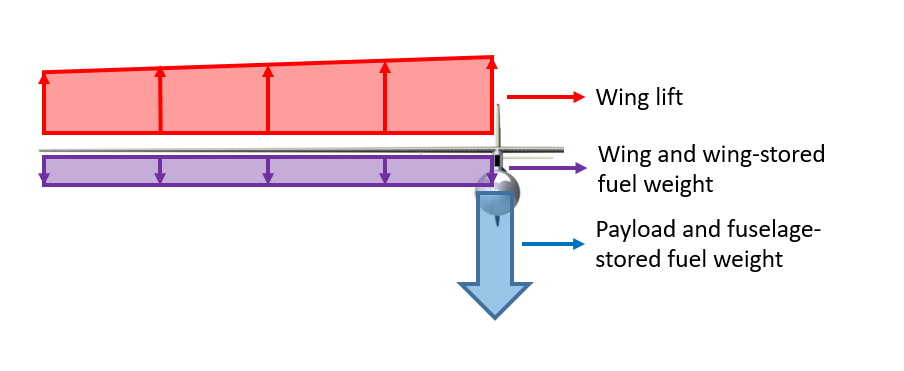
\includegraphics[width=0.8\textwidth]{liftweight.PNG}
\end{figure}

\subsection{Wing Structure}
The wing structure model is based on a simple beam model with a distributed lift load, and a point mass in the center representing the fuselage, as shown in Figure~\ref{fig:liftweight}.

\subsection{Fuel Volume}
The fuel in the aircraft can be stored either in the wing or the fuselage. The signomial constraint in the optimization appears in the fuel volume model, as shown in Equation~\ref{eq:fuel}:

\begin{equation}
\label{eq:fuel}
V_f \leq V_{f_{wing}} + V_{f_{fuse}} 
\end{equation}

where $V_{f_{wing}$ and $V_{f_{fuse}}$ represent the fuel volume available in the wing and the fuselage respectively. They are each represented by the following monomials. 

\begin{equation}
\label{eq:fuelwing}
V_{f_{wing}} <= 9e^{-4}\frac{S^{1.5}\tau}{A^{0.5}}
\end{equation}

\begin{equation}
\label{eq:fuelfuse}
V_{f_{fuse}} <= 10 \times CDA_0~m
\end{equation}

Note that the monomials above are represented with inequalities, to be compatible with the RSP formulation. 

\subsection{Takeoff constraints}
We specify that the aircraft has to be able to takeoff at a speed of $V_{min}$ without exceeding the aircraft stall lift coefficient $C_{L_{max}}$, both of which are specified with an associated uncertainty. 

\section{Uncertainties and sets}

The uncertainties for the different constants in the problem have been determined considering the parameters in aircraft design that often have the largest uncertainty. These uncertainties are listed in Table~\ref{tab:uncertainties}.

\begin{table}
\begin{center}
\caption{\label{tab:uncertainties} Constants and Uncertainties (increasing order)}
\begin{tabular}{c c c c}
\hline
Constant & Description & Value & \% Uncert. ($3\sigma$) \\
$S_{wetratio}$ & wetted area ratio & 2.075 & 3\\
e & span efficiency & 0.92 & 3\\
$\mu$ & viscosity of air & 1.775e-5 kg/(ms) & 4 \\
$\rho$ & air density & 1.23 kg/m^3 & 5 \\
$C_{L_{max}}$ & stall lift coefficient & 1.6 & 5\\
k & fuselage form factor & 1.17 & 10\\
$\tau$ & airfoil thickness ratio & 0.12 & 10\\
$N_{ult}$ & ultimate load factor & 3.3 & 15\\
$V_{min}$ & takeoff speed & 25 m/s & 20\\
$W_0$ & payload weight & 6250 N & 20\\
$W_{w_{coeff1}}$ & wing weight coefficient 1 & 2e-5 1/m & 20\\
$W_{w_{coeff2}}$ & wing weight coefficient 2 & 60 N/m^2 & 20\\
\hline
\end{tabular}
\end{center}
\end{table}

The parameter uncertainties reflect aerospace engineering intuition. The wing weight coefficients $W_{w_{coeff1}}$ and $W_{w_{coeff2}}$, and the ultimate load factor $N_{ult}$ have large $3\sigma$s because build quality of aircraft components often difficult to quantify with a large degree of certainty. The payload weight ($W_0$) has a large uncertainty, because it is valuable if the aircraft has the flexibility to accommodate larger payloads. Parameters that engineers take to be physical constants ($\mu$, $\rho$) and those that can be determined/manufactured with a relatively high degree of accuracy ($S_{wetratio}$, $e$) have relatively low deviations. Parameters that require testing to determine ($C_{L_{max}}$, $V_{min}$) have a level of uncertainty that reflects the expected variance of the parameters. 

\section{Results}

\subsection{Determining the appropriate $\Gamma$}

In this section, we optimize the aircraft configuration for a given payload and range with no uncertainty, box uncertainty and ellipsoidal uncertainty, and attempt to determine the value of $\Gamma$ that gives the best trade-off between robustness and optimality for the RO formulations. The problems have been solved with box uncertainty and ellipsoidal uncertainty for a range of $\Gamma$. For each of the robust solutions, both the estimated probability of failure and the objective cost have been plotted in Figures~\ref{fig:probOfFail_vs_Gamma} and \ref{fig:W_f_vs_Gamma} respectively. 

\begin{figure}[h]
    \centering
    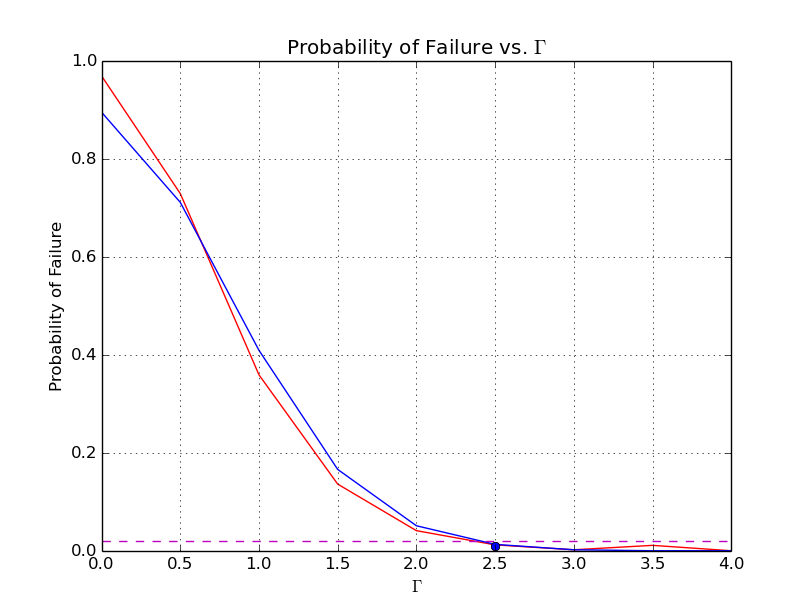
\includegraphics[width=0.6\textwidth]{probOfFail_vs_Gamma.png}
    \caption{The probability of failure vs. $\Gamma$. Note the high ($\geq$ 90\%) probability of failure for the non-robust ($\Gamma$ = 0) solutions. The difference in the probability of failure for the non-robust cases is due to subtle numerical errors in the evaluation of the solution obtained for the ellipsoidal uncertainty set.}
    \label{fig:probOfFail_vs_Gamma}
\end{figure}

\begin{figure}
\centering
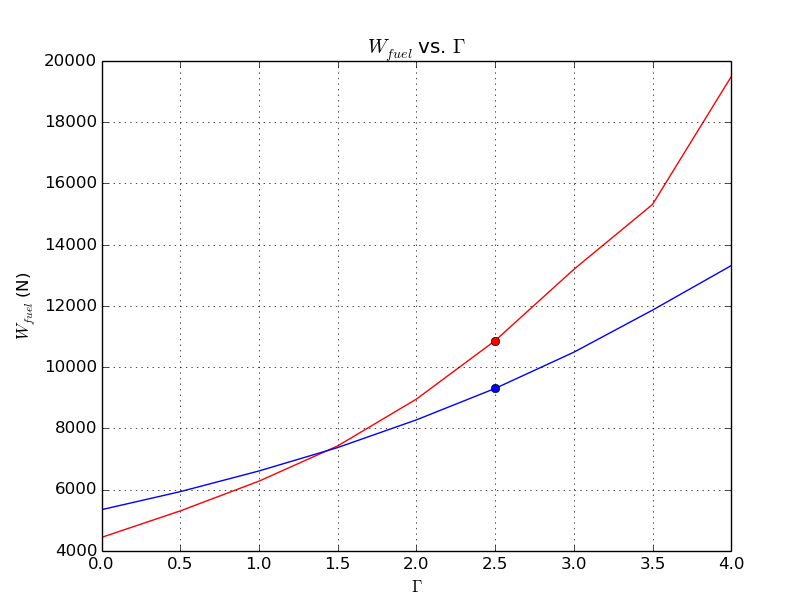
\includegraphics[width=0.6\textwidth]{W_f_vs_Gamma.png}
\caption{Fuel weight vs. $\Gamma$ demonstrates the deterioration of the objective as we protect against larger variation of parameters.}
\label{fig:W_f_vs_Gamma}
\end{figure}

We define the probability of failure to be the probability of constraint violation in 1000 samples of the uncertain parameters from a normal distribution with the specified $3\sigma$ uncertainties. For this problem, we allow for less than 2\% probability of failure, shown by the magenta line in Figure~\ref{fig:probOfFail_vs_Gamma}, and consider half-integer values of $\Gamma$. This corresponds to a $\Gamma$ of 2.5 for both the box uncertainty and the ellipsoidal uncertainty, resulting in 1.2\% and 1.3\% probability of failure respectively.

We know that elliptical uncertainty sets are less conservative than box uncertainty sets, especially when we have a large number of uncertain parameters per constraint. The results we got are somehow expected, and this would show how designing using uncertainty sets is better than using margins which are - in the best case - somehow similar to box uncertainty sets.

\subsection{Optimization results}

At the chosen values of $\Gamma$, the results of the optimization are shown in Table~\ref{tab:results}.

\begin{table}[!h]
\begin{center}
\caption{\label{tab:results} SP Aircraft Optimization Results }
\begin{tabular}{c c c c}
\hline
Free variable & No Uncert. & Box [$\Gamma = 2.5$] & Ellipsoidal [$\Gamma = 2.5$] \\
\hline
$L/D$ & 23.8 & 16.41 & 17.3 \\
$AR$ & 12.0 & 5.016 & 6.56 \\
$Re$ & 4.76e6 & 1.16e7 & 9.55e6 \\
$S (m^2) $ & 21.6 & 72.21 & 58.9 \\
$V (m/s)$ & 51.0 & 47.73 & 48.6 \\ 
$T_{flight} (hr)$ & 17.46 & 18.1 & 17.2 \\
$W_w$ & 2440 & 6278 & 5470 \\
$W_{w_{strc}} (N)$ & 1210 & 1570 & 1650 \\
$W_{w_{surf}} (N)$ & 1230 & 1592 & 3820 \\
$V_{f_{avail}} (m^3)$ & 0.566 & 1.794 & 1.48 \\ 
$V_{f_{fuse}} (m^3)$ & 0.461 & 0.891 & 0.903 \\
$V_{f_{wing}} (m^3)$ & 0.105 & 0.9027 & 0.582 \\
$CDA_0 (m^2)$ & 0.0461 & 0.0891 & 0.0903 \\
\hline
E[Objective] & No Uncert. & Box [$\Gamma = 2.5$] & Ellipsoidal [$\Gamma = 2.5$] \\
\hline
$W_{fuel} $ (N) & 4430 & 10858 & 9299 \\
\hline
P[failure] & No Uncert. & Box [$\Gamma = 2.0$] & Ellipsoidal [$\Gamma = 2.5$] \\
\hline
\% & 92 & 1.2 & 1.3\\
\hline
\end{tabular}
\end{center}
\end{table}

\subsection{Comparing results for different objective functions}

\begin{figure}
\caption{Design optimization of the aircraft with no uncertainty for 3 different objective functions. The red, blue and yellow correspond to $\frac{W_f}{L/D}$, $D$, $W_f$ and objectives respectively.}
\begin{center}
\begin{tikzpicture}[scale=0.75]
\tkzKiviatDiagram{$\frac{W_f}{L/D}$,$D$,$W_f$}
%solve for {W_f}{L/D}
\tkzKiviatLine[thick,
color=red,
mark=ball,
ball color=red,
mark size=3pt,opacity=.2,
fill=red!20](154.4/25,414.2/75,5180/700)
%solve for D
\tkzKiviatLine[thick,
color=blue,
mark=ball,
mark size=3pt,
fill=blue!20,
opacity=.5](161.8/25,400/75,5129/700)
% solve for {W_f}
\tkzKiviatLine[thick,
color=yellow,
mark=ball,
mark size=3pt,
fill= yellow!20,
opacity=.5](190.2/25,463.4/75,4536/700)
\label{fig:spiderplotnoUncert}
\end{tikzpicture}
\end{center}
% tkz-kiviat documentation here in FRENCH: http://mirror.jmu.edu/pub/CTAN/macros/latex/contrib/tkz/tkz-kiviat/doc/TKZdoc-kiviat-main.pdf
\end{figure}

To further demonstrate the capabilities of robust SPs in aircraft design, we performed the optimization of the aircraft with no uncertainty and ellipsoidal uncertainty ($\Gamma = 2.5$) for two more objective functions, and plotted the results on spider plots. Spider plots are useful because they allow engineers to find non-dominated solutions among the solutions that lie on the Pareto frontier of potential objective functions. The objective functions chosen for this analysis were fuel burn over lift-to-drag ratio ($\frac{W_f}{L/D}$), drag ($D$), and fuel burn ($W_f$). 

In the spider plots in Figures \ref{fig:spiderplotnoUncert} and \ref{fig:spiderplotEllUncert}, none of the solutions are non-dominated for both the no uncertainty and ellipsoidal uncertainty cases. In a GP, it is not possible that one of the solutions is non-dominated since the solutions are globally optimal. But since there is no guarantee in optimality for SPs, it is possible to find non-dominated solutions if the obtained solution is a local optimum.

In the case where there is no non-dominated solution such as this one, we take the internal areas of the triangle formed by each optimization to be the figure of merit. The smaller the area in the triangle, the higher the performance of the proposed solution. In the no uncertainty case shown in Figure~\ref{fig:spiderplotnoUncert}, the red solution with the objective of $\frac{W_f}{L/D}$ has the smallest internal area. In the ellipsoidal case shown in Figure~\ref{fig:spiderplotEllUncert}, the blue solution with the objective of $D$ has the smallest internal area. 

This is an interesting result, because the presence of an uncertainty set is shown to affect the efficacy of different objective functions to obtain solutions with the best overall performance. The differences between the objective functions in the simple aircraft design problem are minute, because the different potential objectives have a high degree of coupling. It is likely that, if the three objective functions didn't have high degree of coupling, that the internal areas of the solution triangles may differ more significantly. 

\begin{figure}[H]
\caption{Design optimization of the aircraft with ellipsoidal uncertainty ($\Gamma = 2.5$) for 3 different objective functions. The red, blue and yellow correspond to $\frac{W_f}{L/D}$, $D$, $W_f$ and objectives respectively.}
\begin{center}
\begin{tikzpicture}[scale=0.75]
\tkzKiviatDiagram{$\frac{W_f}{L/D}$,$D$,$W_f$}
%solve for {W_f}{L/D}
\tkzKiviatLine[thick,
color=red,
mark=ball,
ball color=red,
mark size=3pt,opacity=.2,
fill=red!20](568.6/100,1051/150,13500/1500)
%solve for D
\tkzKiviatLine[thick,
color=blue,
mark=ball,
mark size=3pt,
fill=blue!20,
opacity=.5](587/100,1024/150,13100/1500)
% solve for {W_f}
\tkzKiviatLine[thick,
color=yellow,
mark=ball,
mark size=3pt,
fill= yellow!20,
opacity=.5](687.9/100,1155/150,11900/1500)
\label{fig:spiderplotEllUncert}
\end{tikzpicture}
\end{center}
% tkz-kiviat documentation here in FRENCH: http://mirror.jmu.edu/pub/CTAN/macros/latex/contrib/tkz/tkz-kiviat/doc/TKZdoc-kiviat-main.pdf
\end{figure}


\section{Conclusion, and Future Work}

We have developed and applied a tractable RSP formulation to a simple aircraft model, and then discussed the benefits of having robust solutions. RSP formulations extend the tractable approximate RGP framework developed by Saab to non-log-convex problems, and are a valuable contribution to the fields of robust optimization and difference-of-convex programming.\\

RSPs have a wide variety of potential applications in engineering design. Within the Hoburg Research Group in the Aerospace Computational Design Lab, during the past year we have developed a commercial aircraft design SP that has between 1700 and 8000 variables, depending on the whether it is a single-point, or multi-point optimization. We expect that using RO in this conceptual aircraft design will result in designs that are more robust with respect to uncertainties in operational parameters, such as payload mass and range, as well as uncertain constants.

\begin{appendices}

\section{Robust Linear Programming: A Quick Review}

As mentioned earlier, robust linear programming will be used to formulate an approximate robust geometric program.\\[12pt]
Consider the system of linear constraints

\begin{equation*}
    \mat{A}\vec{x} + \vec{b} \leq 0
\end{equation*}

where

\begin{equation*}
\begin{aligned}
\mat{A} &\text{ is $m \times n$}\\
\vec{x} &\text{ is $n \times 1$}\\
\vec{b} &\text{ is $m \times 1$}\\
\end{aligned}
\end{equation*}

where that data is uncertain and is given by equations \eqref{Data} and \eqref{perturbation_set}.

\subsection{Box Uncertainty Set}
If the perturbation set $\mathcal{Z}$ given in equation \eqref{perturbation_set} is a box uncertainty set, i.e. $\|\vec{\zeta}\|_{\infty} \leq \Gamma$, then the robust formulation of the $i^{th}$ constraint is equivalent to
\begin{equation}
\Gamma \textstyle{\sum}_{l=1}^L |- {b}^l_{i} - \vec{a}^l_i\vec{x}| + \vec{a}^0_i\vec{x} + b^0_i \leq 0
\label{box_absolute}
\end{equation}
If only $b$ is uncertain, i.e. $A^l = 0 \quad \forall l = 1,2,...,L$, then equation \eqref{box_absolute} will become
\begin{equation}
\textstyle{\sum}_{l=1}^L \vec{a}^0_{i}\vec{x} + b^0_{i} + \Gamma \textstyle{\sum}_{l=1}^L |b^l_{i}| \leq 0
\label{box_coeff}
\end{equation}
which is a linear constraint\\
On the other hand, if $A$ is uncertain, then equation \eqref{box_absolute} is equivalent to the following set of linear constraints
\begin{equation}
\begin{aligned}
\Gamma \textstyle{\sum}_{l=1}^L w^l_{i} + \vec{a}^0_{i}\vec{x} + b^0_{i} &\leq 0\\
- b^l_{i} - \vec{a}^l_{i}\vec{x} &\leq w^l_{i} &&\forall l \in 1,...,L\\
b^l_{i} + \vec{a}^l_{i}\vec{x} &\leq w^l_{i} &&\forall l \in 1,...,L\\
\end{aligned}
\label{box_linear}
\end{equation}

\subsection{Elliptical Uncertainty Set}
Briefly, if the perturbation set $\mathcal{Z}$ is an elliptical, i.e. $\textstyle{\sum}_{l=1}^L\frac{\zeta_l^2}{\sigma_l^2} \leq \Gamma^2$, then the robust formulation of the $i^{th}$ constraint is equivalent to
\begin{equation}
\Gamma \sqrt{\textstyle{\sum}_{l=1}^L \sigma_l^2(- b^l_{i} - \vec{a}^l_{i}\vec{x})^2} + \vec{a}^0_{i}\vec{x} + b^0_{i} \leq 0
\label{ell_absolute}
\end{equation}
which is a second order conic constraint.\\
If only $b$ is uncertain, i.e. $\mat{A}^l = 0 \quad \forall l = 1,2,...,L$, then equation \eqref{ell_absolute} will become
\begin{equation}
\textstyle{\sum}_{l=1}^L \vec{a}^0_{i}\vec{x} + b^0_{i} + \Gamma \sqrt{\textstyle{\sum}_{l=1}^L \sigma_l^2(b^l_{i})^2} \leq 0
\label{ell_coeff}
\end{equation}
which is a linear constraint.
\subsection{Norm-1 Uncertainty Sets}
Briefly, if the perturbation set represented by $\mathcal{Z}$ is a norm-1 uncertainty set, i.e. $\|\vec{\zeta}\|_1 \leq \Gamma$, then the robust constraint is
\begin{equation}
\textstyle{\sum}_{l=1}^L \vec{a}^0_{i}\vec{x} + b^0_{i} + \Gamma \max_{l=1,..,L} |b^l_{i}| \leq 0
\label{rom_coeff}
\end{equation}
when $\mat{A}^l = 0$, and 
\begin{equation}
\begin{aligned}
\Gamma w_{i} + \vec{a}^0_{i}\vec{x} + b^0_{i} &\leq 0\\
- b^l_{i} - \vec{a}^l_{i}\vec{x} &\leq w_{i} &&\forall l \in 1,...,L\\
b^l_{i} + \vec{a}^l_{i}\vec{x} &\leq w_{i} &&\forall l \in 1,...,L\\
\end{aligned}
\label{rom_linear}
\end{equation}
if $\mat{A}^l \neq 0$\\
Note that for this type of uncertainty, the robust constraints are linear.

\end{appendices}

\end{document}
